%!TEX root = ../thesis.tex
\mychapter{Literature Study}{Literature Study}{}
\label{chap:literature}

\mysection{Language models as robot task planners}{Language Models as Robot Task Planners}
\label{sec:llm_planners}

Large language models carry a great deal of general knowledge about the world, but that
knowledge is not grounded in what any particular robot can actually do. An LLM asked to
``tidy the kitchen'' has plenty to say about what tidying a kitchen involves, and none of it
accounts for whether the robot in front of it has an arm, what that arm can reach, or whether
``the sponge'' refers to something the robot has ever seen. To Close the gap, connecting the
model's reasoning to a specific robot's actual capabilities, is what the systems in this
section have in common, even though they close it in different ways.

SayCan \cite{ahn2022saycan} grounds the model by constraining its output rather than trusting
it outright. The LLM proposes a set of candidate next actions drawn from a fixed library of
pretrained skills, but each candidate is re-scored by a separately learned affordance function.
that estimates how likely that skill is to succeed given the robot's current state. The action
that is both something the LLM would suggest and something the robot can plausibly do is the
one that gets executed. Grounding, in this framing, is a second model checking the first, not
something the LLM is trusted to know on its own.



Code as Policies \cite{liang2023codeaspolicies} takes a different route. Rather than picking
from a fixed skill library, the LLM writes code, calling perception functions, control
primitives, and other functions it has been shown examples of, composed however the
instruction requires. This lets it handle instructions no one anticipated in advance and
assign precise parameters (a velocity, a threshold) to descriptions that were only ever given
in words, at the cost of needing a language model capable of writing correct, composable code
rather than just picking from a short list.

Inner Monologue \cite{huang2023innermonologue} addresses a limitation both of the above still
have: a plan committed to once, before anything happens, has no way to adapt as the situation
unfolds. It closes the loop by feeding the robot's ongoing observations, success and failure
signals, scene descriptions, even a human's spoken interjection, back into the language
model's own reasoning process, so it can revise what it does next in light of what actually
happened rather than what it expected to happen.

None of these three were built for tasks longer than about ten actions. Hori et al.\ \cite{hori2025longhorizon} target that gap directly, arguing that long-horizon tasks fail for a different reason than short ones: the command usually leaves out information the model would need to plan the whole thing correctly, and no amount of re-scoring or code generation fixes a plan built on a wrong assumption. Their method resolves this through what they call active
modification, the model asks clarifying questions before committing to a plan, combined with
passive modification, refining the plan afterwards against visual feedback. This is the most
direct ancestor of the clarification loop this project builds: extending plan length by first
closing the information gap in the command, rather than by making the underlying model larger or its skill library richer.
\begin{figure}[H]
    \centering
    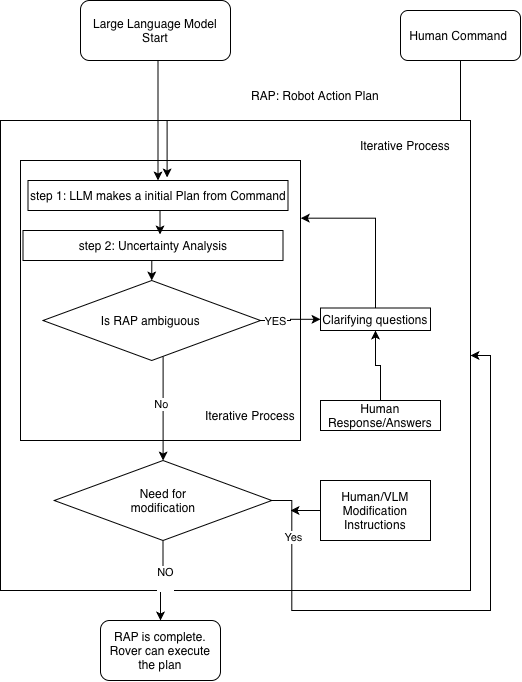
\includegraphics[width=0.8\linewidth]{figures/figure1.drawio.png}
    \caption{Process overview of RAP generation before rover departures}
    \label{fig:your_label}
\end{figure}

Last point Code as Policies'
approach assumes a language model capable of writing correct, composable code against a rich API, which is a reasonable assumption for a cloud-hosted model that has more computing power but not for the small, locally hosted planner this project depends on for RQ1.

\mysection{Grounding plans in a bounded action set}{Grounding Plans in a Bounded Action Set}
\label{sec:grounding}

SayCan and Code as Policies set the standard way to connect an LLM's plan to what a robot can
actually do. SayCan~\cite{ahn2022saycan} pairs the LLM with a separately learned value function for
each robot skill. The language model scores how relevant an action sounds for the instruction. The
value function scores whether the robot can do it right now. The two scores are combined, so the
action picked is both sensible and physically possible. Figure~\ref{fig:saycan_scoring} shows this
with a concrete instruction, "how would you put an apple on the table?" The LLM alone ranks
\emph{find an apple}, \emph{find a coke}, and \emph{find a sponge} almost the same, since all three
are plausible first steps for some task. The value function breaks that tie: \emph{find an apple}
and the other two score identically on the language side, but only the apple is actually visible in
the robot's current scene, so the combined score, log-probability from the LLM multiplied against
the affordance probability, pushes it to the top of the list. Nothing about the instruction told the
model an apple was present. The value function is what supplied that.

\begin{figure}[H]
    \centering
    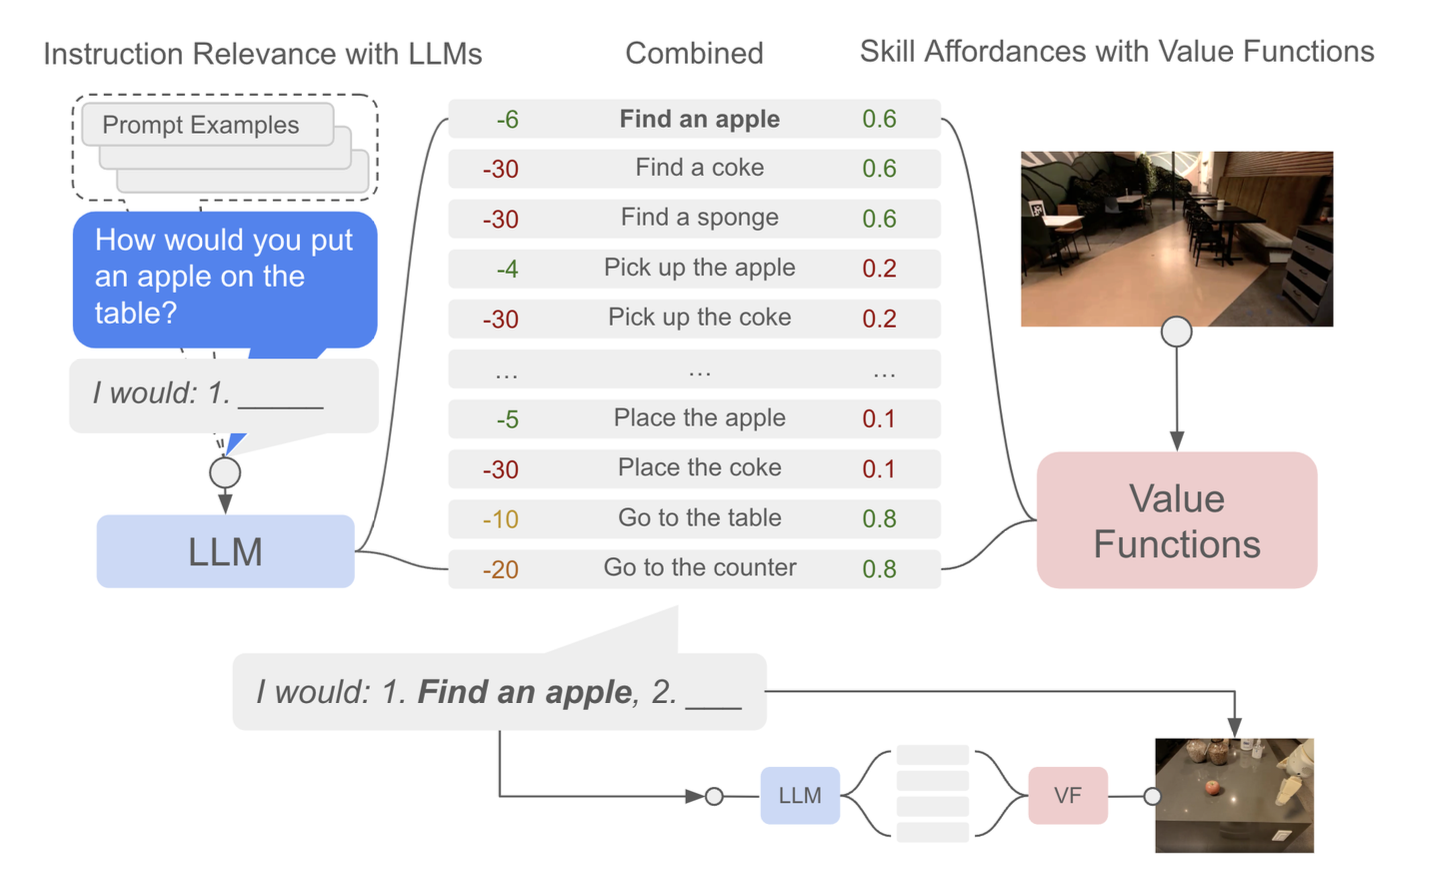
\includegraphics[width=0.85\linewidth]{figures/saycan_scoring.png}
    \caption{SayCan combining language-model relevance scores with value-function affordance
    scores to select the next skill, reproduced from Ahn et al.~\cite{ahn2022saycan}.}
    \label{fig:saycan_scoring}
\end{figure}

Ahn et al. formalise this selection rule as

\begin{equation}
    \operatorname*{arg\,max}_{\pi \in \Pi} \mskip\thickmuskip p(c_\pi \mid s, \ell_\pi) \, p(\ell_\pi \mid i)
    \label{eq:saycan_selection}
\end{equation}

where:
$\Pi$ is the set of available skill  

$\ell_\pi$ is skill $\pi$'s textual label, 

$i$ is the instruction, 

$s$ is the current state,

$c_\pi$ is the event that $\pi$ completes successfully.

$p(\ell_\pi \mid i)$ is task-grounding, the language model's estimate of how well a skill matches the
instruction, and $p(c_\pi \mid s, \ell_\pi)$ is world-grounding, the value function's estimate of
whether that skill would succeed from the current state. 

These are exactly the two columns in
Figure~\ref{fig:saycan_scoring}, the LLM's log-probabilities are $\log p(\ell_\pi \mid i)$, and the
0.6/0.2/0.1/0.8 values are $p(c_\pi \mid s, \ell_\pi)$.

Code as Policies~\cite{liang2023codeaspolicies} solves the same problem a different way: the LLM
writes Python that calls a fixed set of perception and control functions directly. If the code does
not compile against that API, the step cannot run.

Both approaches give the planner a fixed set of actions it cannot go outside of. This project's
capability vocabulary in \texttt{planner.py} plays the same role: a step whose target or action
falls outside that vocabulary is rejected rather than passed through to the rover.

Neither approach checks what happens after a step runs. Inner Monologue~\cite{huang2023innermonologue}
adds that check on top of a SayCan-style setup: after each action, the robot gets an observation
back, a success or failure signal, a scene description, or something the human said, and the next
step is planned using that observation instead of the original plan alone. Plan a step, act, observe,
replan. This project's mid-mission execution follows the same loop: each frame sent over
\texttt{/ws/execution} is what the plan gets checked against after each step, not only before the
mission starts, allowing the plan to respond to drift the rover has actually accumulated rather than
committing to a path decided before departure.


\mysection{Clarification and ambiguity}{Clarification and ambiguity in human-robot interaction}
\label{sec:clarification_lit}

A spoken instruction only resolves to a single rover action if the rover's 
observations rule out every other reading of it. "Bring the bowl" is unambiguous with one bowl on the counter 
and ambiguous with two. \citet{hori2025longhorizon} describe two ways to correct a task plan once this kind of ambiguity shows up: 
passive modification, where a person reviews the plan and 
points out what is wrong, and active modification, where the planner judges its own uncertainty and asks a question before acting. 

Passive modification is accurate, since a human checks every step, but it is repetitive. The plan has to be re-issued and re-checked 
each time something is off. Active modification moves that judgment onto the model, so the human is only asked to step in when the model is actually unsure.

\citet{ren2023knowno} give active modification a statistical guarantee, in a method called KnowNo, and \citeauthor{hori2025longhorizon} cite it directly as a working example of the approach. 
KnowNo does not let the planner commit to its single highest-scoring next step. The planner's raw confidence scores for each candidate step are passed through a conformal prediction layer, 
which converts them into a calibrated set of steps that are all plausible enough to keep. A singleton set means the rover proceeds on its own. A set with more than one step means the instruction was ambiguous 
given what the rover can observe, and the rover asks a clarifying question instead of guessing. Figure~\ref{fig:knowno_pipeline} shows the example used in the paper. It is told to place the bowl in the microwave with a metal and a plastic bowl both on the counter, 
the two matching steps score close enough that neither clears the calibrated threshold on its own, so the system asks which one, plastic or metal, instead of picking one.

\begin{figure}[H]
    \centering
    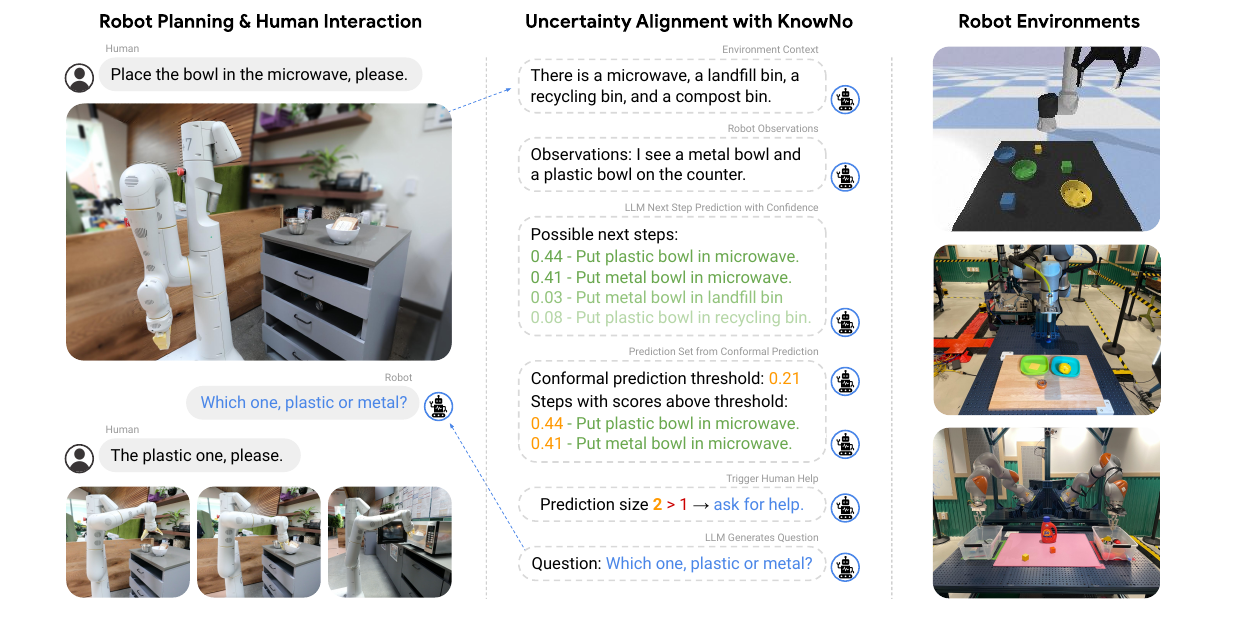
\includegraphics[width=0.95\linewidth]{figures/knowno_prediction_set.png}
    \caption{The KnowNo pipeline: an LLM planner proposes next steps with confidence scores, conformal prediction narrows these to a calibrated prediction set, and the rover asks for help whenever that set contains more than one option. Reproduced from \citet{ren2023knowno}.}
    \label{fig:knowno_pipeline}
\end{figure}

The calibration works as follows. Given a held-out calibration set of $N$ examples, 
each with a true label $y_i$ and a model score $\hat{f}(\tilde{x}_i)_{y_i}$ for that label, 
a nonconformity score is computed for every example:

\begin{equation}
    \kappa_i = 1 - \hat{f}(\tilde{x}_i)_{y_i}.
    \label{eq:knowno_score}
\end{equation}

The calibrated threshold $\hat{q}$ is then set to the

\begin{equation}
    \frac{\lceil (N+1)(1-\epsilon) \rceil}{N} \text{ empirical quantile of } \kappa_1, \dots, \kappa_N,
    \label{eq:knowno_quantile}
\end{equation}

where $\epsilon$ is a user-chosen error tolerance. At test time, the prediction set kept for a new instruction is every label whose score clears this threshold:

\begin{equation}
    C(\tilde{x}_{\text{test}}) = \left\{ y \in Y \mskip\thickmuskip\middle|\mskip\thickmuskip \hat{f}(\tilde{x}_{\text{test}})_y \geq 1-\hat{q} \right\}.
    \label{eq:knowno_predset}
\end{equation}

Conformal prediction guarantees that this set contains the correct label with the user-specified probability,

\begin{equation}
    P\big(y_{\text{test}} \in C(\tilde{x}_{\text{test}})\big) \geq 1-\epsilon.
    \label{eq:knowno_coverage}
\end{equation}

This guarantee is what makes the threshold usable in practice: instead of picking a confidence cut-off 
by hand and hoping it behaves sensibly, the rover's decision to act alone comes with a stated bound on how 
often that decision is correct.


\mysection{Locally hosted models}{Locally hosted and quantised models}
\label{sec:local_models}

Sections~\ref{sec:llm_planners} to \ref{sec:clarification_lit} assume the rover can call out to a large, cloud-hosted LLM. A rover cannot always guarantee that access: network connectivity is not 
reliable in every test environment, and the round-trip latency to a cloud endpoint works against the response time a voice-commanded system needs to feel usable. Running the planner locally, 
on hardware the rover carries itself, removes both problems, but restricts the model to whatever fits in on-board memory.

Quantisation is the standard technique for making a model fit that constraint: model weights, and in some cases activations, are stored using fewer bits than the 16 or 32 bits used at training time, 
at some cost to numerical precision. \citet{liu2025quantreasoning} define uniform quantisation of a tensor $\mathbf{X}$ to $b$ bits as

\begin{equation}
    \hat{\mathbf{X}} = \mathcal{Q}(\mathbf{X}; b) = s \cdot \Pi_{\Omega(b)}\mskip-\thinmuskip\left(\frac{\mathbf{X}}{s}\right), \qquad s = \frac{\max(\mathbf{X}) - \min(\mathbf{X})}{2^{b}-1},
    \label{eq:quantization}
\end{equation}

where 
\begin{itemize}[font=\bfseries]
    \item $\Omega(b) = \{0, 1, \dots, 2^{b}-1\}$ is the set of representable integer levels
    \item $\Pi_{\Omega(b)}(\cdot)$ rounds to the nearest one.
\end{itemize}

This is applied at different bit-widths for weights and activations, written for example as W8A8 (8-bit weights, 8-bit activations) or W4A16 (4-bit weights, 16-bit activations); A lower bit-width gives a smaller model and a coarser step size $s$, and therefore more rounding error per value.

\citet{husom2025edgellm} benchmark quantised LLMs directly on 
edge hardware and report that quantisation lowers energy use and inference 
latency substantially, at a small cost to output accuracy on straightforward tasks. \citet{liu2025quantreasoning} show 
that this cost is not constant across task types. Accuracy degrades faster as bit-width drops on tasks that require 
chaining several reasoning steps together than on single-step tasks. The planning step described in Section~\ref{sec:llm_planners} 
is exactly that kind of multi-step reasoning task, so the bit-width chosen for a locally hosted planner in this project is not only an 
efficiency setting. It is a direct trade-off against how reliably the planner reasons through a multi-step voice command.

\mysection{Compositional depth and hallucination}{Compositional depth and hallucination}
\label{sec:hallucination_lit}

The methods discussed in Sections~\ref{sec:llm_planners} to \ref{sec:clarification_lit} treat each planning step largely on its own. 
As a task plan grows longer and more compositional, two further problems appear that a single-step clarification mechanism does not cover: the LLM's reasoning can degrade over a long chain of steps, 
producing a confidently stated plan that is simply wrong, and the rover can encounter a scene it was never prepared for, one that no single faulty component causes 
but that the plan as a whole fails to account for.

\citet{liang2024introspective} address the first problem by extending the conformal prediction procedure from Section~\ref{sec:clarification_lit} with a retrieval step. Rather than scoring each candidate plan from the LLM's raw confidence alone, 
their method, introspective planning, 
first builds a knowledge base of worked examples. For a given task and observation, an LLM is prompted to explain in writing why certain candidate actions are 
valid and others are not. At deployment, the system retrieves the most similar past example by embedding similarity and includes it in the prompt before the LLM scores its candidates, 
as shown in Figure~\ref{fig:introspective_pipeline}. Grounding each new decision in a similar, explained precedent sharpens the confidence scores that conformal prediction operates on,
which produces the same statistically guaranteed prediction set from Equations~\ref{eq:knowno_predset}--\ref{eq:knowno_coverage} while asking the user fewer unnecessary questions.

\begin{figure}[H]
    \centering
    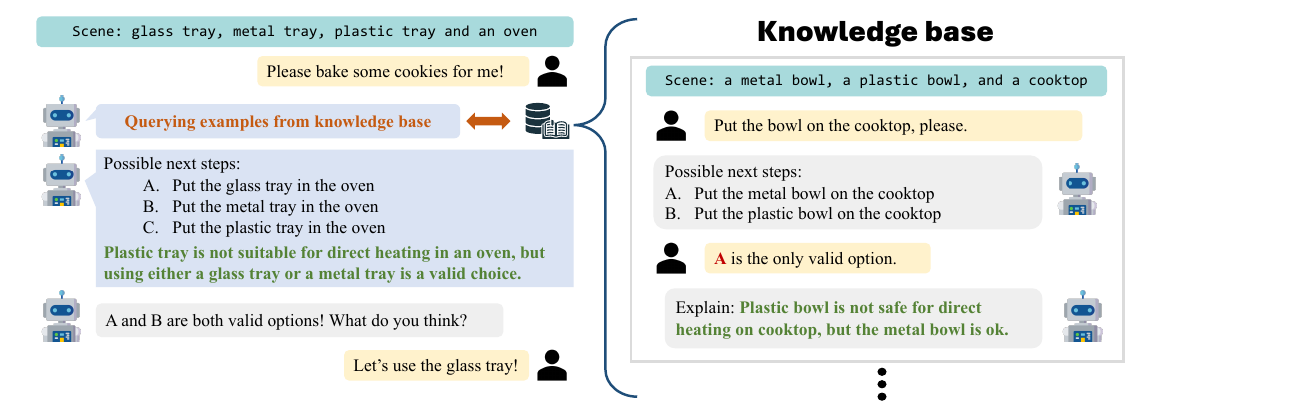
\includegraphics[width=0.95\linewidth]{figures/introspective_planning_pipeline.png}
    \caption{The introspective planning pipeline: a knowledge base of explained past examples is built offline, and at deployment the most similar example is retrieved to inform the LLM's confidence for each candidate step. Reproduced from \citet{liang2024introspective}.}
    \label{fig:introspective_pipeline}
\end{figure}

The second problem, an unanticipated scene rather than an unreliable plan, 
is addressed by \citet{sinha2024aesop} and \citet{elhafsi2023semantic} from the
 direction of runtime monitoring rather than planning. \citeauthor{sinha2024aesop} propose a 
 two-stage monitor: a fast binary classifier screens every observation in an LLM embedding space, 
 and only when it flags a possible anomaly does a slower, more capable LLM reason explicitly about 
 what has gone wrong and which fallback plan to switch to. Splitting the monitor this way keeps the fast 
 path cheap enough to run continuously, while reserving the expensive reasoning step for the moments it is 
 actually needed, which matters directly for a rover with the limited on-board compute discussed in 
 Section~\ref{sec:local_models}. \citeauthor{elhafsi2023semantic} apply the same idea of an LLM as a 
 monitor to what they term semantic anomalies. A system-level failures, like an autonomous vehicle
  braking for a stop sign printed on a billboard. That does not come from any single broken component, but 
  from a gap in the system's contextual reasoning.

Together, these three methods extend the single-step clarification of 
Section~\ref{sec:clarification_lit} along a different axis: introspective planning 
improves the confidence estimate feeding a single decision, while AESOP and semantic anomaly 
detection catch failures a confidence score never gets the chance to be wrong about, because the
 plan itself is being carried out against a scene the planner misjudged.

\mysection{Speech recognition for local languages}{Speech recognition for South African English and Afrikaans}
\label{sec:stt_lit}

Every method discussed so far assumes the instruction $d_i$ handed to 
the LLM planner is already correct text. For a voice-commanded rover, that 
text comes from a speech-to-text stage first, and an error there becomes an error in the 
planner's input before any clarification mechanism gets a chance to act 
on it. South African English and Afrikaans are both under-represented in the training data of general-purpose
 speech recognisers, which makes this an upstream risk specific to a South African test environment.

\citet{kamper2012multiaccent} quantify how much accent variation costs a algorthmn used for recognising speech, trained 
without accounting for accent variation. Working with 31.78 hours of speech across five South African 
English accents (Afrikaans English, Black South African English, Cape Flats English, White South 
African English, and Indian South African English), they compare three acoustic modelling strategies: a separate model per accent, 
a single model pooling all accents together, and a multi-accent model that shares acoustic structure across accents 
where it helps while keeping accent-specific distinctions where it does not. The multi-accent model reached 82.78\% word accuracy, 
against 81.53\% for accent-specific models and 81.52\% for a single pooled model, a difference the authors report as statistically significant. 
Black South African English stood out as the one accent that still benefited from being modelled separately rather than pooled, which the authors attribute to it being acoustically the most distinct of the five.

\citet{jacobs2025afrikaans} work at the opposite end of the resource spectrum: fine-tuning Whisper on Afrikaans and isiXhosa oral narratives 
spoken by four- and five-year-old children, using only five minutes of transcribed in-domain child speech. They find that adding in-domain adult speech, 
especially combined with voice conversion to make it sound more child-like, gives the largest accuracy gain of any strategy tried, and that parameter-efficient 
fine-tuning helps Afrikaans but not isiXhosa, since isiXhosa is more severely under-represented in Whisper's original training data.

Together, these results point at the same conclusion from different directions. 
Local accents and languages measurably degrade off-the-shelf speech recognition, and the fix in both cases is not more general-purpose training data but a small, targeted amount of in-domain or in-accent data. 
For a rover meant to take spoken commands from South African English or Afrikaans speakers, this is a design constraint on the speech-to-text stage that sits upstream of every planning method discussed in
Sections~\ref{sec:llm_planners} to~\ref{sec:hallucination_lit}, not something those methods can correct for after the fact.

\mysection{Research gap}{Research gap}
\label{sec:gap}

Sections~\ref{sec:llm_planners} to \ref{sec:stt_lit} cover five separate strands of work: grounding an LLM's plan in what a rover can actually do (Sections~\ref{sec:llm_planners}-\ref{sec:grounding}), 
asking for clarification when an instruction is genuinely ambiguous (Section~\ref{sec:clarification_lit}), catching the failures that a confidence score alone will not (Section~\ref{sec:hallucination_lit}), 
running the planner on hardware small enough for a rover to carry (Section~\ref{sec:local_models}), and recognising speech accurately in a South African accent or language (Section~\ref{sec:stt_lit}).
Each strand has been developed and evaluated largely on its own.

The methods in Sections~\ref{sec:clarification_lit} and \ref{sec:hallucination_lit} that provide statistical guarantees on plan correctness, KnowNo and introspective planning, are demonstrated with large, 
cloud-hosted LLMs. Section~\ref{sec:local_models} shows that quantisation, needed to run a planner locally, costs accuracy disproportionately on exactly the kind of multi-step reasoning these planners perform, 
but neither \citet{ren2023knowno} nor \citet{liang2024introspective} evaluate their calibration procedure on a quantised, locally hosted model. Whether a conformal prediction threshold calibrated on a full-precision 
model still gives a valid guarantee once that model is quantised down to fit on-board memory is not addressed by either strand of work.

Similarly, none of the planning or clarification methods in Sections~\ref{sec:llm_planners} to \ref{sec:hallucination_lit} are evaluated with speech input, let alone speech in a South African accent or in Afrikaans. 
Section~\ref{sec:stt_lit} shows that accent and language mismatch measurably degrades transcription accuracy, which means an instruction $d_i$ reaching the planner in this project's setting carries a source of error the literature above does not model at all. 
An ambiguity introduced by a transcription error is not the same problem as an ambiguity in the underlying instruction, and it is unclear from the existing literature whether a clarification mechanism designed for the latter behaves sensibly when faced with the former.

This project sits at the intersection of these gaps: a voice-commanded indoor rover that must plan and clarify using a locally hosted, quantised LLM, taking speech input from South African English or Afrikaans speakers. No single work reviewed in this chapter evaluates this combination, and the remainder of this report investigates how the planning, clarification, and speech recognition 
components described above hold up once combined on hardware a rover runs on.
